%%%%%%%%%%%%%%%%%%%%%%%%%%%%%%%%%%%%%%%%%
% Beamer Presentation
% LaTeX Template
% Version 1.0 (10/11/12)
%
% This template has been downloaded from:
% http://www.LaTeXTemplates.com
%
% License:
% CC BY-NC-SA 3.0 (http://creativecommons.org/licenses/by-nc-sa/3.0/)
%
%%%%%%%%%%%%%%%%%%%%%%%%%%%%%%%%%%%%%%%%%

%----------------------------------------------------------------------------------------
%	PACKAGES AND THEMES
%----------------------------------------------------------------------------------------

\documentclass{beamer}

\mode<presentation> {

% The Beamer class comes with a number of default slide themes
% which change the colors and layouts of slides. Below this is a list
% of all the themes, uncomment each in turn to see what they look like.

%\usetheme{default}
%\usetheme{AnnArbor}
%\usetheme{Antibes}
%\usetheme{Bergen}
%\usetheme{Berkeley}
%\usetheme{Berlin}
%\usetheme{Boadilla}
%\usetheme{CambridgeUS}
%\usetheme{Copenhagen}
%\usetheme{Darmstadt}
%\usetheme{Dresden}
%\usetheme{Frankfurt}
%\usetheme{Goettingen}
%\usetheme{Hannover}
%\usetheme{Ilmenau}
%\usetheme{JuanLesPins}
%\usetheme{Luebeck}
\usetheme{Madrid}
%\usetheme{Malmoe}
%\usetheme{Marburg}
%\usetheme{Montpellier}
%\usetheme{PaloAlto}
%\usetheme{Pittsburgh}
%\usetheme{Rochester}
%\usetheme{Singapore}
%\usetheme{Szeged}
%\usetheme{Warsaw}

% As well as themes, the Beamer class has a number of color themes
% for any slide theme. Uncomment each of these in turn to see how it
% changes the colors of your current slide theme.

%\usecolortheme{albatross}
%\usecolortheme{beaver}
%\usecolortheme{beetle}
%\usecolortheme{crane}
%\usecolortheme{dolphin}
%\usecolortheme{dove}
%\usecolortheme{fly}
%\usecolortheme{lily}
%\usecolortheme{orchid}
%\usecolortheme{rose}
%\usecolortheme{seagull}
%\usecolortheme{seahorse}
%\usecolortheme{whale}
%\usecolortheme{wolverine}

%\setbeamertemplate{footline} % To remove the footer line in all slides uncomment this line
%\setbeamertemplate{footline}[page number] % To replace the footer line in all slides with a simple slide count uncomment this line

%\setbeamertemplate{navigation symbols}{} % To remove the navigation symbols from the bottom of all slides uncomment this line
}

\usepackage{graphicx} % Allows including images
\usepackage{booktabs} % Allows the use of \toprule, \midrule and \bottomrule in tables

%----------------------------------------------------------------------------------------
%	TITLE PAGE
%----------------------------------------------------------------------------------------

\title[Short title]{Finite difference method for 1D time independent Schr\"{o}dinger equations } % The short title appears at the bottom of every slide, the full title is only on the title page

\author{Xiaofeng Xu} % Your name
\institute[HKUST] % Your institution as it will appear on the bottom of every slide, may be shorthand to save space
{
Hong Kong University of Science and Technology \\ % Your institution for the title page
\medskip
\textit{xxuam@connect.ust.hk} % Your email address
}
\date{\today} % Date, can be changed to a custom date

\begin{document}

\begin{frame}
\titlepage % Print the title page as the first slide
\end{frame}

\begin{frame}
\frametitle{Overview} % Table of contents slide, comment this block out to remove it
\tableofcontents % Throughout your presentation, if you choose to use \section{} and \subsection{} commands, these will automatically be printed on this slide as an overview of your presentation
\end{frame}

%----------------------------------------------------------------------------------------
%	PRESENTATION SLIDES
%----------------------------------------------------------------------------------------

%------------------------------------------------
\section{First Section} % Sections can be created in order to organize your presentation into discrete blocks, all sections and subsections are automatically printed in the table of contents as an overview of the talk
%------------------------------------------------

\subsection{Subsection Example} % A subsection can be created just before a set of slides with a common theme to further break down your presentation into chunks
\begin{frame}{Overview}
Modified Kronig Penneys are studied to understand band gap of crystal and localization of eigenstates in disordered systems by solving the Schr\"{o}dinger equation numerically. 
\begin{itemize}
    \item Under the modified Kronig Penney model, how does the band structure look like and how does bad gap relate to potentials at atom sites
    \item We introduce some randomness to our modified Kronig Penny models and then compare the probability density functions and study factors affecting localization. 
\end{itemize}
\end{frame}




\begin{frame}
\frametitle{Background}
In solid state physics, every solid has its own characteristic electronic band structure(diagram) on which there is so called valence band and conduction band. 
\begin{itemize}
    \item Band gap is the energy difference between the top of the valence band and bottom of the conduction band
    \item In order to promote valence electrons to conduction electron, energy is required to overcome the band gap 
    \item Band gap is a major factor determining the electrical conductivity of a solid
    \item Thus, it is important to understand factors that affects band gap
\end{itemize}
Task: Electronic band structures are usually associated with crystalline materials, so in 1D,  we will be looking at a chain of atom with periodic potential and study the band gap. 

\end{frame}

\begin{frame}{Background}
    
    \begin{block}{ Time independent Schr\"{o}dinger equation}
    \begin{equation} \label{eq:2.1}
-\frac{d^2\psi}{dx^2}+V(x)\psi=E\psi              
\end{equation}
\end{block}

    \begin{block}{ Probability density function}
    \begin{equation} \label{eq:2}
    \rho (x) = |\psi(x)|^2
\end{equation}
\end{block}
\begin{block}{Goal}
Numerically solve this equation to get the eigenstates with coresponding eigenvalues and compute the probability density function to study localization of eigenstates

\end{block}

\end{frame}

\begin{frame}{Background}
    From now on, for clearer organization, we separate the study of band gap and localization of eigenstates into two models in this presentation. 
    \newline
    Because although the physical models share some similarities but the physical phenomena we are look at are different in these two situations.
\end{frame}


%------------------------------------------------

\begin{frame}
\frametitle{Model 1 for studying band gap}
\begin{figure}
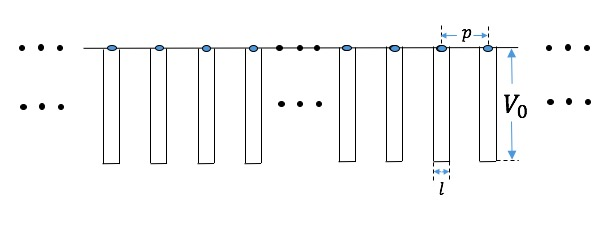
\includegraphics[width=0.8\linewidth]{kp_bandgap.jpeg}
\end{figure}
An infinite chain of atoms with non-overlapping negative square well potentials. For numerical computation, We will confine ourselves to a chain of N atoms with periodic boundary conditions. 
\end{frame}

\begin{frame}{Bloch theorem}
    We could have simply computed the eigenvalues by numerically solving the Schrodinger equations directly. We can then study the distribution of eigenvalues to see if there is any gap somewhere. 
    Recall that we only consider a sample of $N$ atoms with periodic boudary condition, i.e. $\psi(x+Np) = \psi(x)$. 
    \newline
    Under these conditions, Bloch theorem tells us that the solution would be of the form $$\psi_k(x) = e^{i{\alpha_k}x}u_k(x),$$ 
    with $u_k(0) = u_k(p)$,
    and $\alpha_k$ taking values (Note that $\alpha_k$ is called the wave vector)
    $$\alpha_k = \frac{x\pi k}{Np}, \quad k = -\frac{Np}{2},...,\frac{Np}{2}. $$
    After substituting it into Schrodinger equation, we can get
\begin{equation}\label{eq:2.2bloch}
-\frac{1}{2}(\frac{d}{dx}+i\alpha_k)^2u_k+V(x)u_k = Eu_k
\end{equation}
    
\end{frame}

\begin{frame}{Numerical solution: Converting to a finite dimensional eigenvalue problem}
    \begin{block}{Schr\"{o}dinger equation -- Bloch theorem version}
   \begin{equation}\label{eq:2.2bloch}
-\frac{1}{2}(\frac{d}{dx}+i\alpha_k)^2u_k+V(x)u_k = Eu_k
\end{equation}
\end{block}
For each wave vector $\alpha_k$, we solve the equation for eigenvalues and plot the eigenvalues against the wave vectors. This gives us the band structure and then we can compute the band gap.  

    \begin{block}{Equivalent form}
   \begin{equation}\label{eq:expand}
-\frac{1}{2}\frac{d^2u_k}{dx^2}-i\alpha_k \frac{d u_k}{dx} +\frac{1}{2}{\alpha_k}^2u_k+V(x)u_k = Eu_k
\end{equation}
\end{block}

\end{frame}

\begin{frame}{Numerical solution continued ...}

We discretize the interval for this problem into a sequence of equally spaced points $\{x_n\}_{n = 0,1,...,N}$. Then we have the following equations:
\begin{align*} 
 -\frac{1}{2}\frac{d^2u_k(x_0)}{dx^2}-i\alpha_k \frac{d u_k(x_0)}{dx} +\frac{1}{2}{\alpha_k}^2u_k(x_0)+V(x_0)u_k(x_0)  &= Eu_k(x_0)  \\
  -\frac{1}{2}\frac{d^2u_k(x_1)}{dx^2}-i\alpha_k \frac{d u_k(x_1)}{dx} +\frac{1}{2}{\alpha_k}^2u_k(x_1)+V(x_1)u_k(x_1)  &= Eu_k(x_1) \\
......\\
 -\frac{1}{2}\frac{d^2u_k(x_N)}{dx^2}-i\alpha_k \frac{d u_k(x_N)}{dx} +\frac{1}{2}{\alpha_k}^2u_k(x_N)+V(x_N)u_k(x_N)  &= Eu_k(x_N) \\
\end{align*}
\end{frame}

\begin{frame}{Numerical solution continued ...}
    \begin{block}{Centered finite difference scheme for differential operators}
    For convenience, we drop the subscrip $k$ in previous equations.
    \begin{align*} 
\frac{d^2u(x_i)}{dx^2} & \approx \frac{u(x_{i-1})-2u(x_i)+u(x_{i+1}))}{2h^2} \\
\frac{du(x_i)}{dx} & \approx \frac{u(x_{i+1})-u(x_{i-1})}{2h}
\end{align*}
\end{block}

We plug in the above two approximations and apply the periodic boundary condition. After rearranging, we get the following: 

\begin{block}{After approximation using centered fintie difference}
$$(-\frac{1}{2h^2}+\frac{i\alpha}{2h})u_{i-1} + (\frac{1}{h^2}+\frac{1}{2}\alpha^2+V_i)u_i+(-\frac{1}{2h^2}-\frac{i\alpha}{2h})u_{i+1} = Eu_i  $$
\end{block}

\end{frame}

\begin{frame}{Numerical solution continued ...}
\begin{block}{Matrix form}

\begin{equation} 
\left[ \begin{matrix}
\frac{1}{h^2}+\frac{1}{2}\alpha+V_0 & -\frac{1}{2h^2}-\frac{i\alpha}{2h} & & -\frac{1}{2h^2}+\frac{i\alpha}{2h}\\
-\frac{1}{2h^2}+\frac{i\alpha}{2h} & \ddots & \ddots & \\
& \ddots & \ddots & -\frac{1}{2h^2}-\frac{i\alpha}{2h} \\
-\frac{1}{2h^2}-\frac{i\alpha}{2h} & & -\frac{1}{2h^2}+\frac{i\alpha}{2h} & \frac{1}{h^2}+\frac{1}{2}\alpha+V_{N} \end{matrix} \right]
\begin{bmatrix}
    u_{0}  \\
    u_{1}  \\
    \vdots  \\
    u_{N-1}\\
    u_{N}
    \end{bmatrix} = E\begin{bmatrix}
    u_{0}  \\
    u_{1}  \\
    \vdots  \\
    u_{N-1}\\
    u_{N}
    \end{bmatrix}
\end{equation}

\end{block}

The above matrix can be solved using python eigenvalue solver to obtain the eigenvalues. 
Note for each wave vector, we obtain such a matrix. Hence, we need to solve matrices for all wave vectors. 

\end{frame}

\begin{frame}{Examples of band structure plotted}
\begin{columns}[c] % The "c" option specifies centered vertical alignment while the "t" option is used for top vertical alignment

\column{.45\textwidth} % Left column and width
\begin{figure}
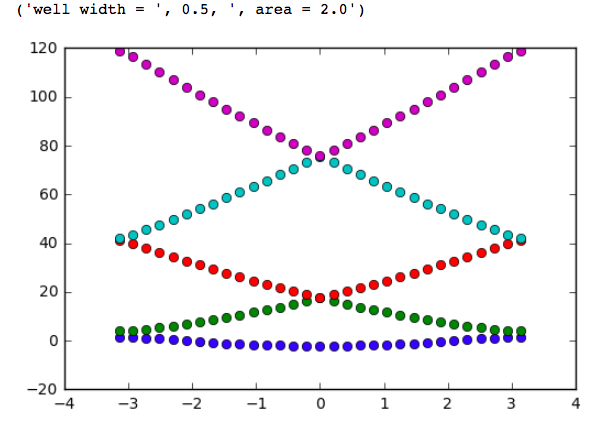
\includegraphics[width=0.8\linewidth]{bandstructure1.png}
\end{figure}

\column{.5\textwidth} % Right column and width
\begin{figure}
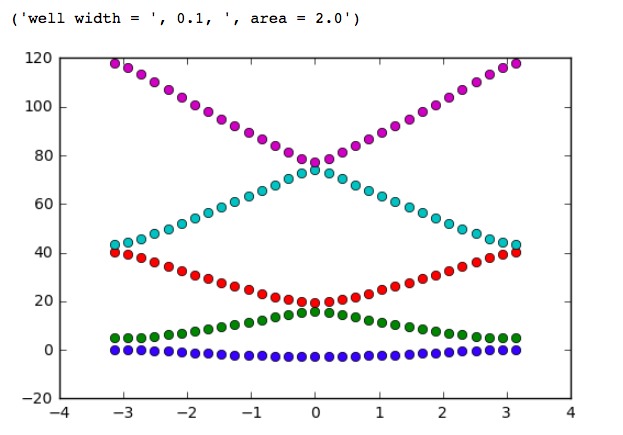
\includegraphics[width=0.8\linewidth]{bandstructure2.png}
\end{figure}

\end{columns}

\end{frame}
\begin{frame}{What we have investigated}
We want to see what changes would make to the band gap if we modify the potentials at atom sites. 
\begin{enumerate}
    \item We fix the well width for the potential and vary the potential height. 
    \item We fix the potential height and vary the well width. 
\end{enumerate}

\end{frame}

\begin{frame}{Results}
\begin{itemize}
    \item Vary potential heights at different fixed well width
\end{itemize}
\begin{figure}
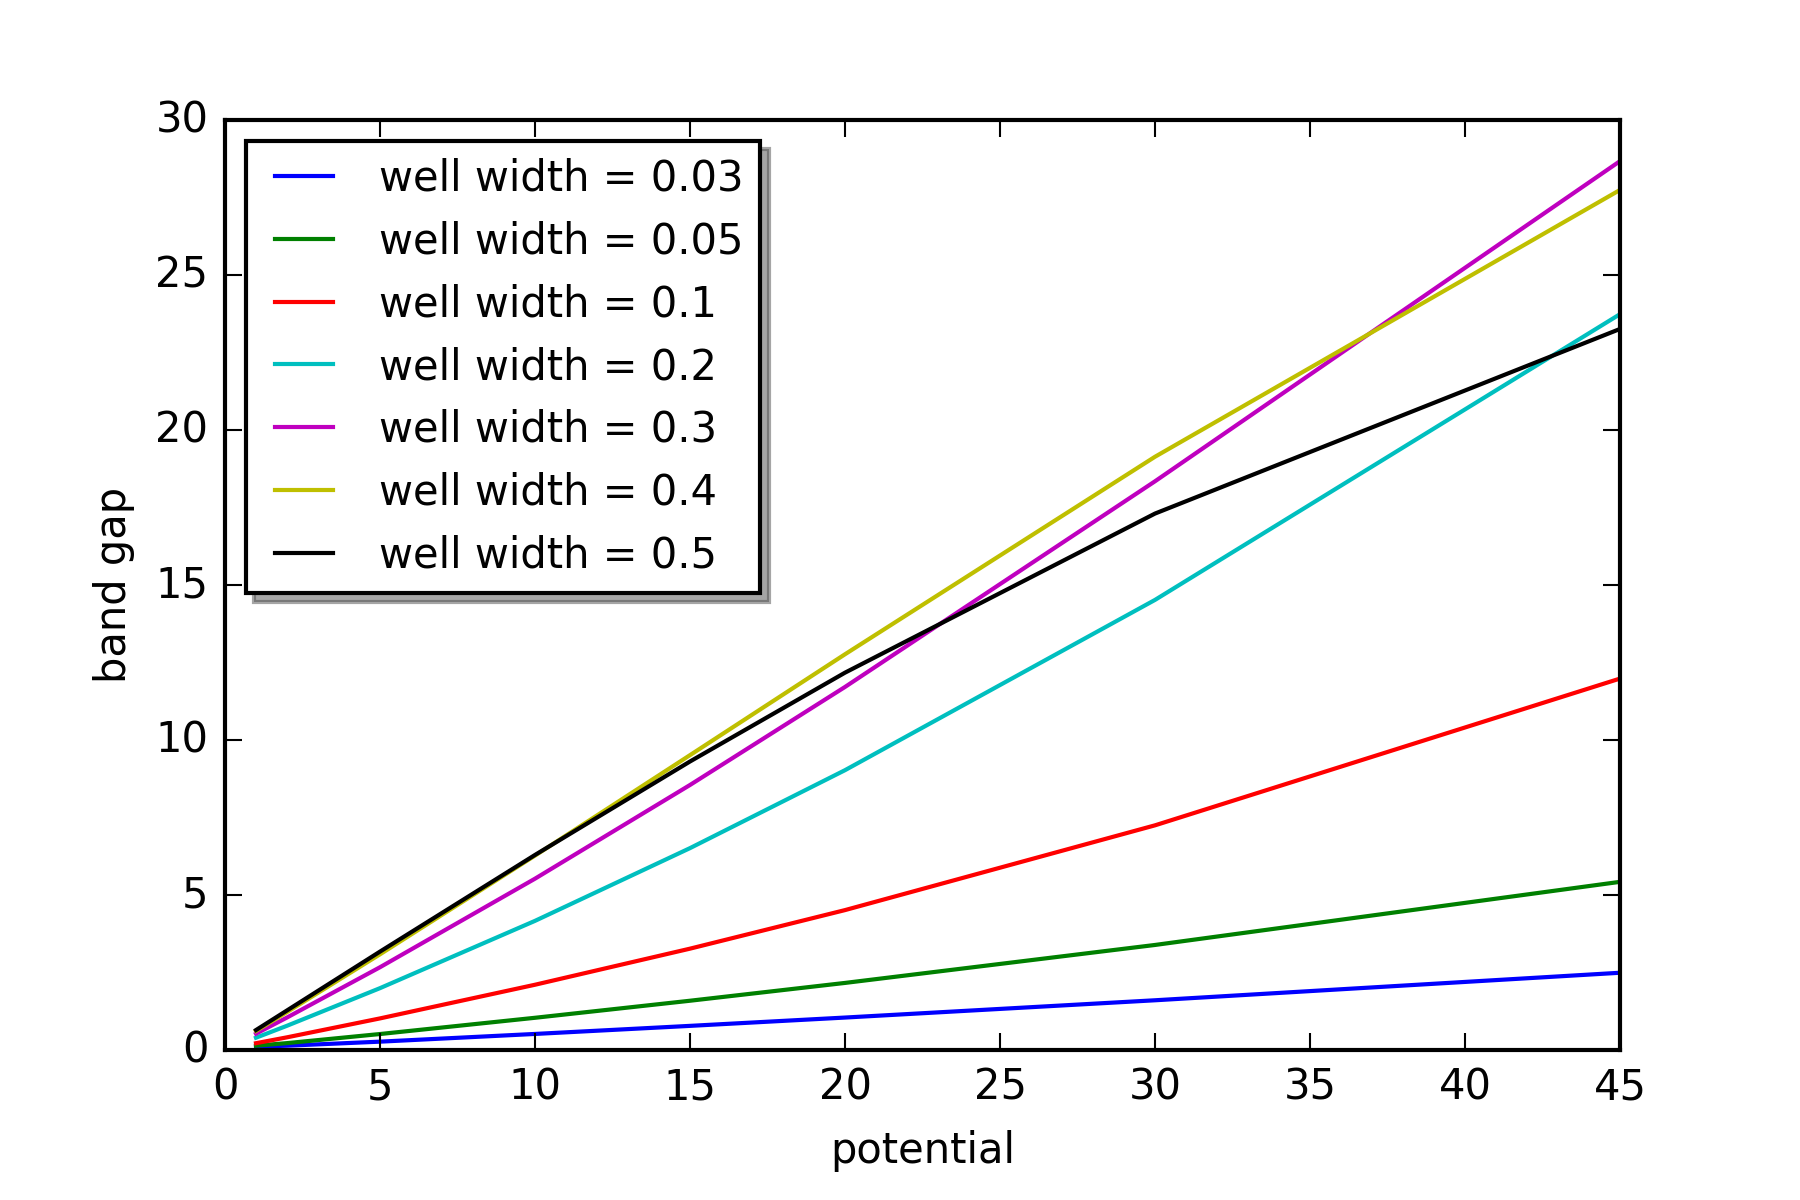
\includegraphics[width=0.8\linewidth]{potentialHeights.png}
\caption{band gap against potential heights at fixed well widths}
\end{figure}
\end{frame}

\begin{frame}{Results}
\begin{itemize}
    \item Vary well width at different fixed potential heights
\end{itemize}
\begin{figure}
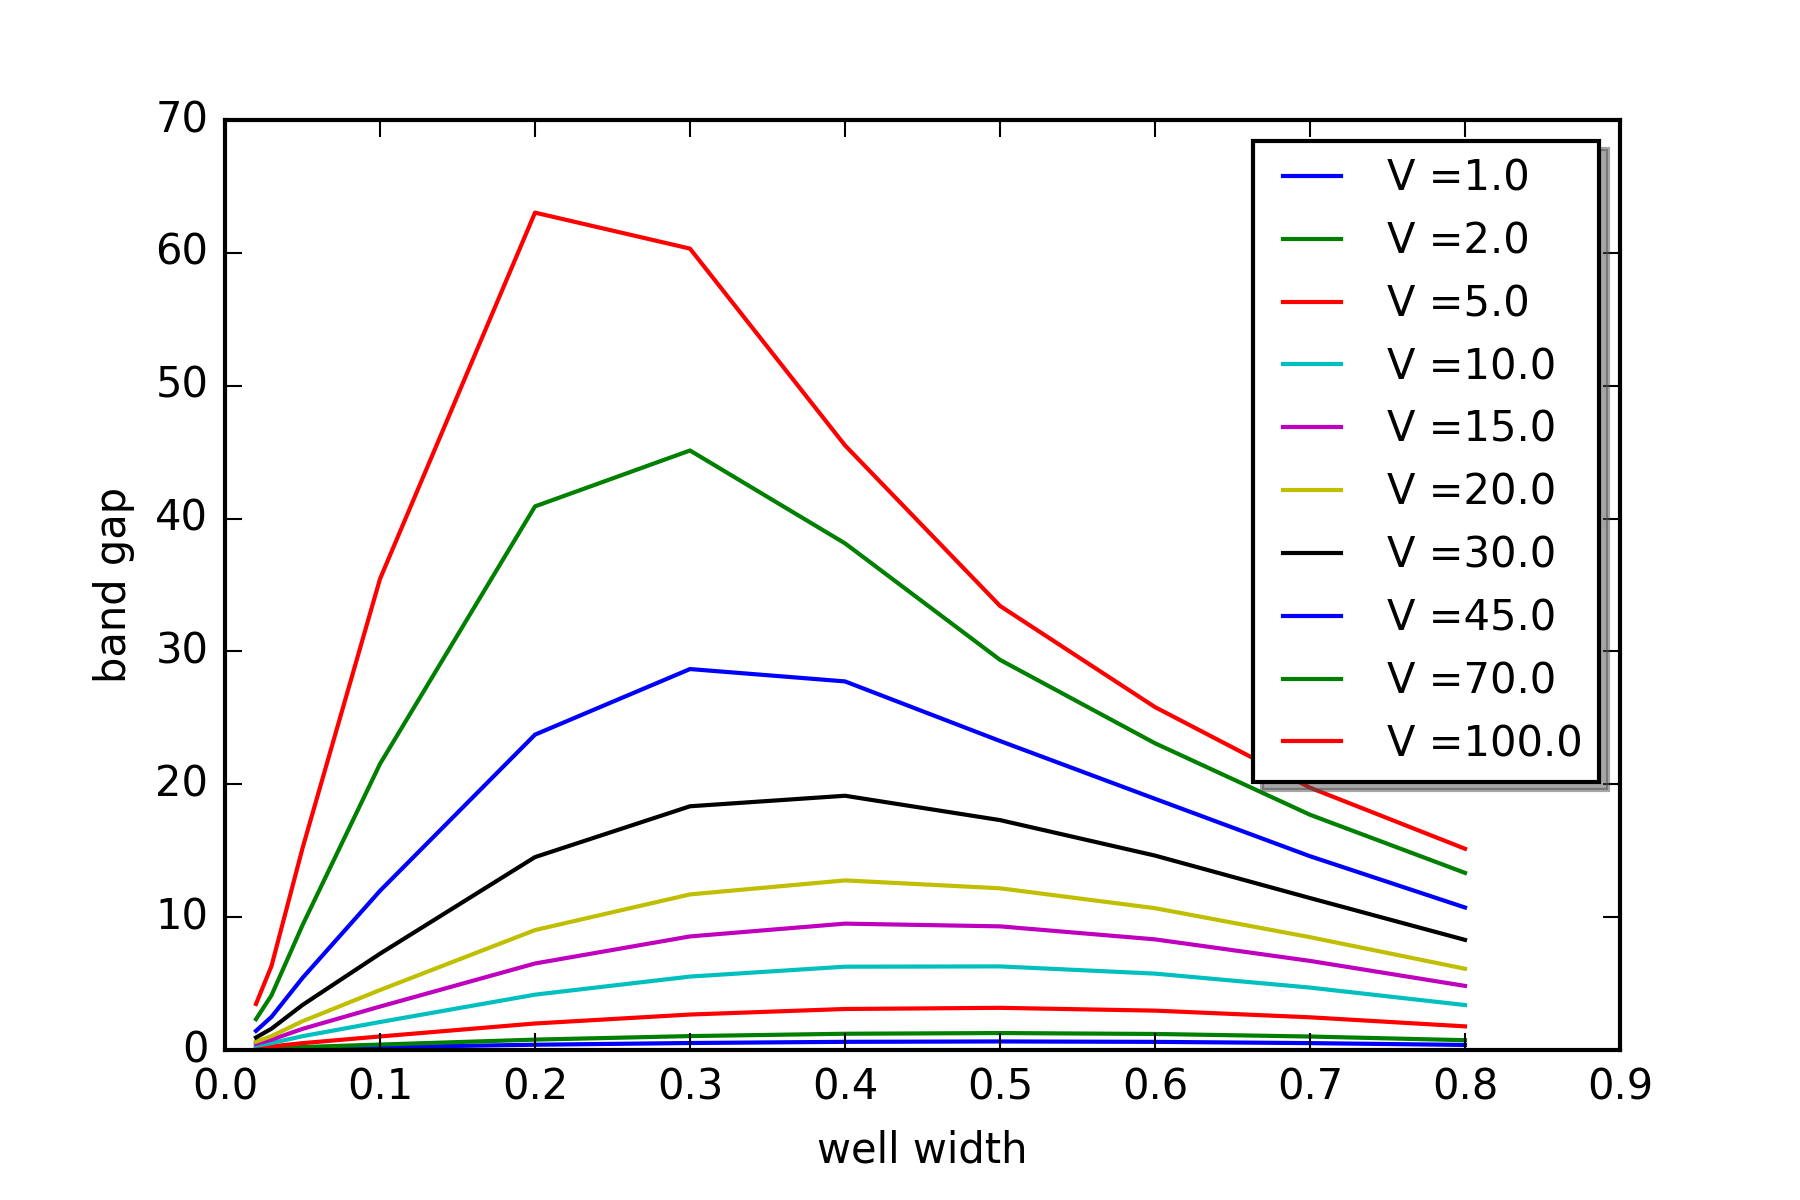
\includegraphics[width=0.8\linewidth]{changeWell.png}
\caption{band gap against well widths at fixed potential heights}
\end{figure}
\end{frame}

\begin{frame}{Conclusion and Discussion}

\begin{enumerate}
    \item The band gap increases when the potential height increases at a fixed well width as we can see from the above figures.  This matches with our intuition that when the electron is trapped in deeper wells, it leads to a larger band gap. 
    \item When fixing the potential, we see that the band gap increases and then decreases as well width increases, resulting in a peak midway. 
    Intuitively, the peak could be understood by considering two extreme cases
    
\end{enumerate}


\end{frame}

\begin{frame}
\frametitle{Model 2 for localization of eigenstates(wavefunction)}

\begin{figure}
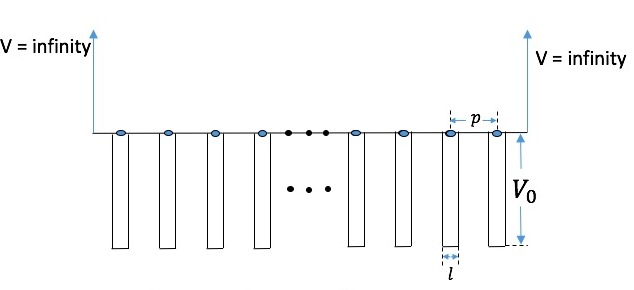
\includegraphics[width=0.8\linewidth]{square_potential_problem.jpeg}
\end{figure}

A chain of atoms with non-overlapping negative square well potentials. We impose zero boundary conditions for the wave function. So the potential at two end is positive infinity.

\end{frame}

\begin{frame}{Introducing randomness to potentials in model 2}
1. Randomness in atomic spacing
\begin{itemize}
    \item spacing between 2 atoms take a value from \{$a_1$,$a_2$\} with probability  \{$P(a_1)$,$P(a_2)$\}. 
\end{itemize}

Notice the potential at each atom site can be determined by potential well width and potential height, the product of which give the area. 
\newline
2. Randomness in potential 
\begin{itemize}
    \item Fixing the area, the well width takes a value from \{$w_1$,$w_2$\} with probability  \{$P(w_1)$,$P(w_2)$\}.
\end{itemize}

    
\end{frame}

%------------------------------------------------

\begin{frame}
\frametitle{Blocks of Highlighted Text}
\begin{block}{Block 1}
Lorem ipsum dolor sit amet, consectetur adipiscing elit. Integer lectus nisl, ultricies in feugiat rutrum, porttitor sit amet augue. Aliquam ut tortor mauris. Sed volutpat ante purus, quis accumsan dolor.
\end{block}

\begin{block}{Block 2}
Pellentesque sed tellus purus. Class aptent taciti sociosqu ad litora torquent per conubia nostra, per inceptos himenaeos. Vestibulum quis magna at risus dictum tempor eu vitae velit.
\end{block}

\begin{block}{Block 3}
Suspendisse tincidunt sagittis gravida. Curabitur condimentum, enim sed venenatis rutrum, ipsum neque consectetur orci, sed blandit justo nisi ac lacus.
\end{block}
\end{frame}

%------------------------------------------------

\begin{frame}
\frametitle{Multiple Columns}
\begin{columns}[c] % The "c" option specifies centered vertical alignment while the "t" option is used for top vertical alignment

\column{.45\textwidth} % Left column and width
\textbf{Heading}
\begin{enumerate}
\item Statement
\item Explanation
\item Example
\end{enumerate}

\column{.5\textwidth} % Right column and width
Lorem ipsum dolor sit amet, consectetur adipiscing elit. Integer lectus nisl, ultricies in feugiat rutrum, porttitor sit amet augue. Aliquam ut tortor mauris. Sed volutpat ante purus, quis accumsan dolor.

\end{columns}
\end{frame}

%------------------------------------------------
\section{Second Section}
%------------------------------------------------

\begin{frame}
\frametitle{Table}
\begin{table}
\begin{tabular}{l l l}
\toprule
\textbf{Treatments} & \textbf{Response 1} & \textbf{Response 2}\\
\midrule
Treatment 1 & 0.0003262 & 0.562 \\
Treatment 2 & 0.0015681 & 0.910 \\
Treatment 3 & 0.0009271 & 0.296 \\
\bottomrule
\end{tabular}
\caption{Table caption}
\end{table}
\end{frame}

%------------------------------------------------

\begin{frame}
\frametitle{Theorem}
\begin{theorem}[Mass--energy equivalence]
$E = mc^2$
\end{theorem}
\end{frame}

%------------------------------------------------

\begin{frame}[fragile] % Need to use the fragile option when verbatim is used in the slide
\frametitle{Verbatim}
\begin{example}[Theorem Slide Code]
\begin{verbatim}
\begin{frame}
\frametitle{Theorem}
\begin{theorem}[Mass--energy equivalence]
$E = mc^2$
\end{theorem}
\end{frame}\end{verbatim}
\end{example}
\end{frame}

%------------------------------------------------

\begin{frame}
\frametitle{Figure}
Uncomment the code on this slide to include your own image from the same directory as the template .TeX file.
%\begin{figure}
%\includegraphics[width=0.8\linewidth]{test}
%\end{figure}
\end{frame}

%------------------------------------------------

\begin{frame}[fragile] % Need to use the fragile option when verbatim is used in the slide
\frametitle{Citation}
An example of the \verb|\cite| command to cite within the presentation:\\~

This statement requires citation \cite{p1}.
\end{frame}

%------------------------------------------------

\begin{frame}
\frametitle{References}
\footnotesize{
\begin{thebibliography}{99} % Beamer does not support BibTeX so references must be inserted manually as below
\bibitem[Smith, 2012]{p1} John Smith (2012)
\newblock Title of the publication
\newblock \emph{Journal Name} 12(3), 45 -- 678.
\end{thebibliography}
}
\end{frame}

%------------------------------------------------

\begin{frame}
\Huge{\centerline{The End}}
\end{frame}

%----------------------------------------------------------------------------------------

\end{document}